
\documentclass[runningheads]{llncs}
\usepackage[text={150mm,220mm},centering]{geometry}
\usepackage{graphicx}
\usepackage{tikz}
\usepackage{float}
\begin{document}
\title{\large{CSCI814 IT Project Management (Lab1)}}
%--------------------Please do NOT change the content above.-------------------------------------------------

%
%----Please write your personal information as below.------------------------------------
%
\author{\large{Student Name: Wangzhihui Mei \\ % Please write your name here
CCNU Student Number: 2019124044 \\ % Please write your CCNU student number here
UOW Student Number: 6603385}}  % Please write your UOW student number here


%-----------------------------------------------------------------------------------------------



%---------Do not change the content of this part--------------------

\authorrunning{CCNU Wollongong Joint Institute}
\institute{Central China Normal University Wollongong Joint Institute}

\maketitle


%-----------Please write your solutions to the questions in the assignment from here.---------------

\section{In-class exercise}

\begin{figure}[H]
    \centering
    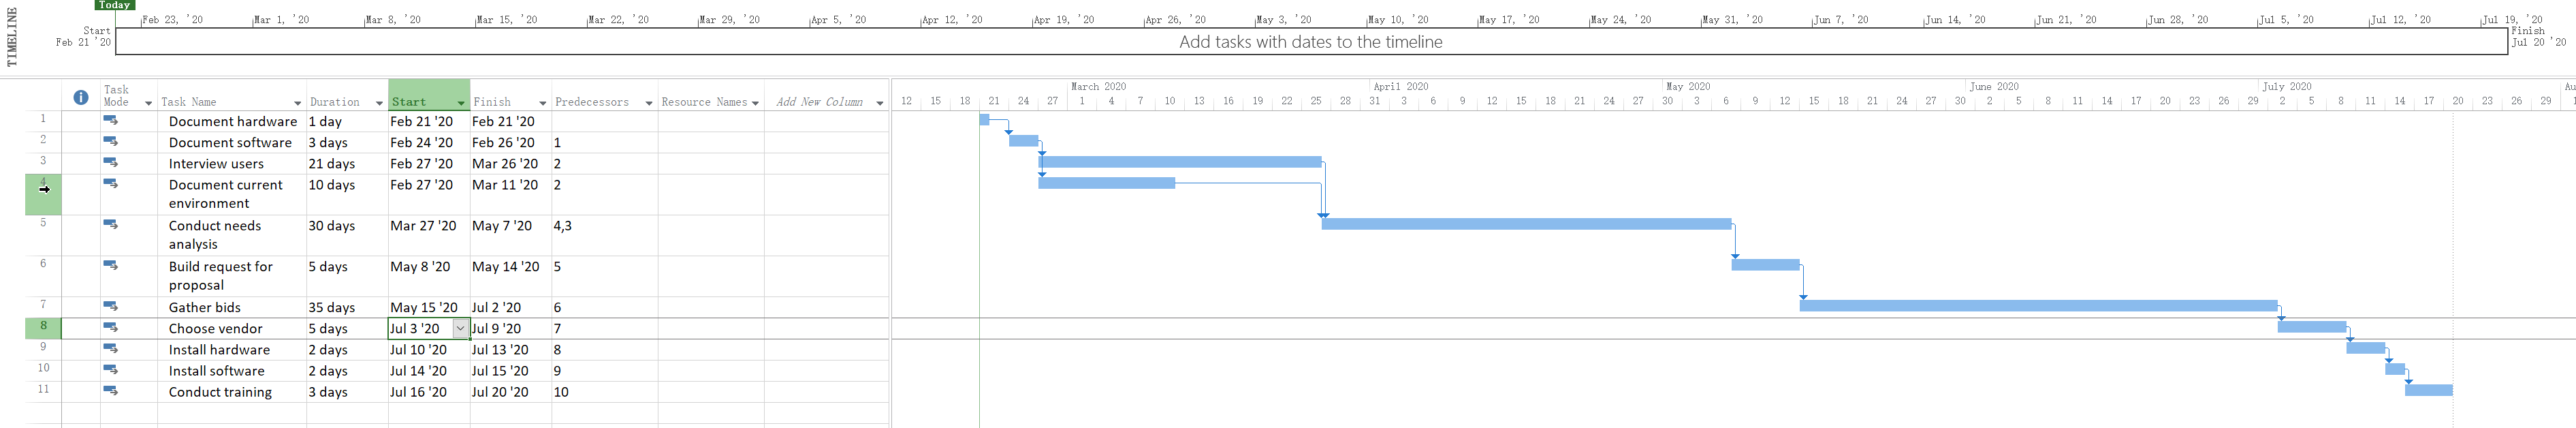
\includegraphics[width=1.0\textwidth]{./image/proj1}
    \caption{Gantt Chart 1}
\end{figure}

\noindent2) The former tasks are the prerequisite of the following tasks.

\noindent3) Timeline: Feb. 21 - Jul. 20, 151 days in total (considering weekends)

\noindent4) Jul. 16, The 147th day of the project

\noindent5) It won't affect the project completion date

\noindent6) Jul. 23, an additional weekend will be included in the timeline.

\noindent7,8,9,10) 
\begin{figure}[H]
    \centering
    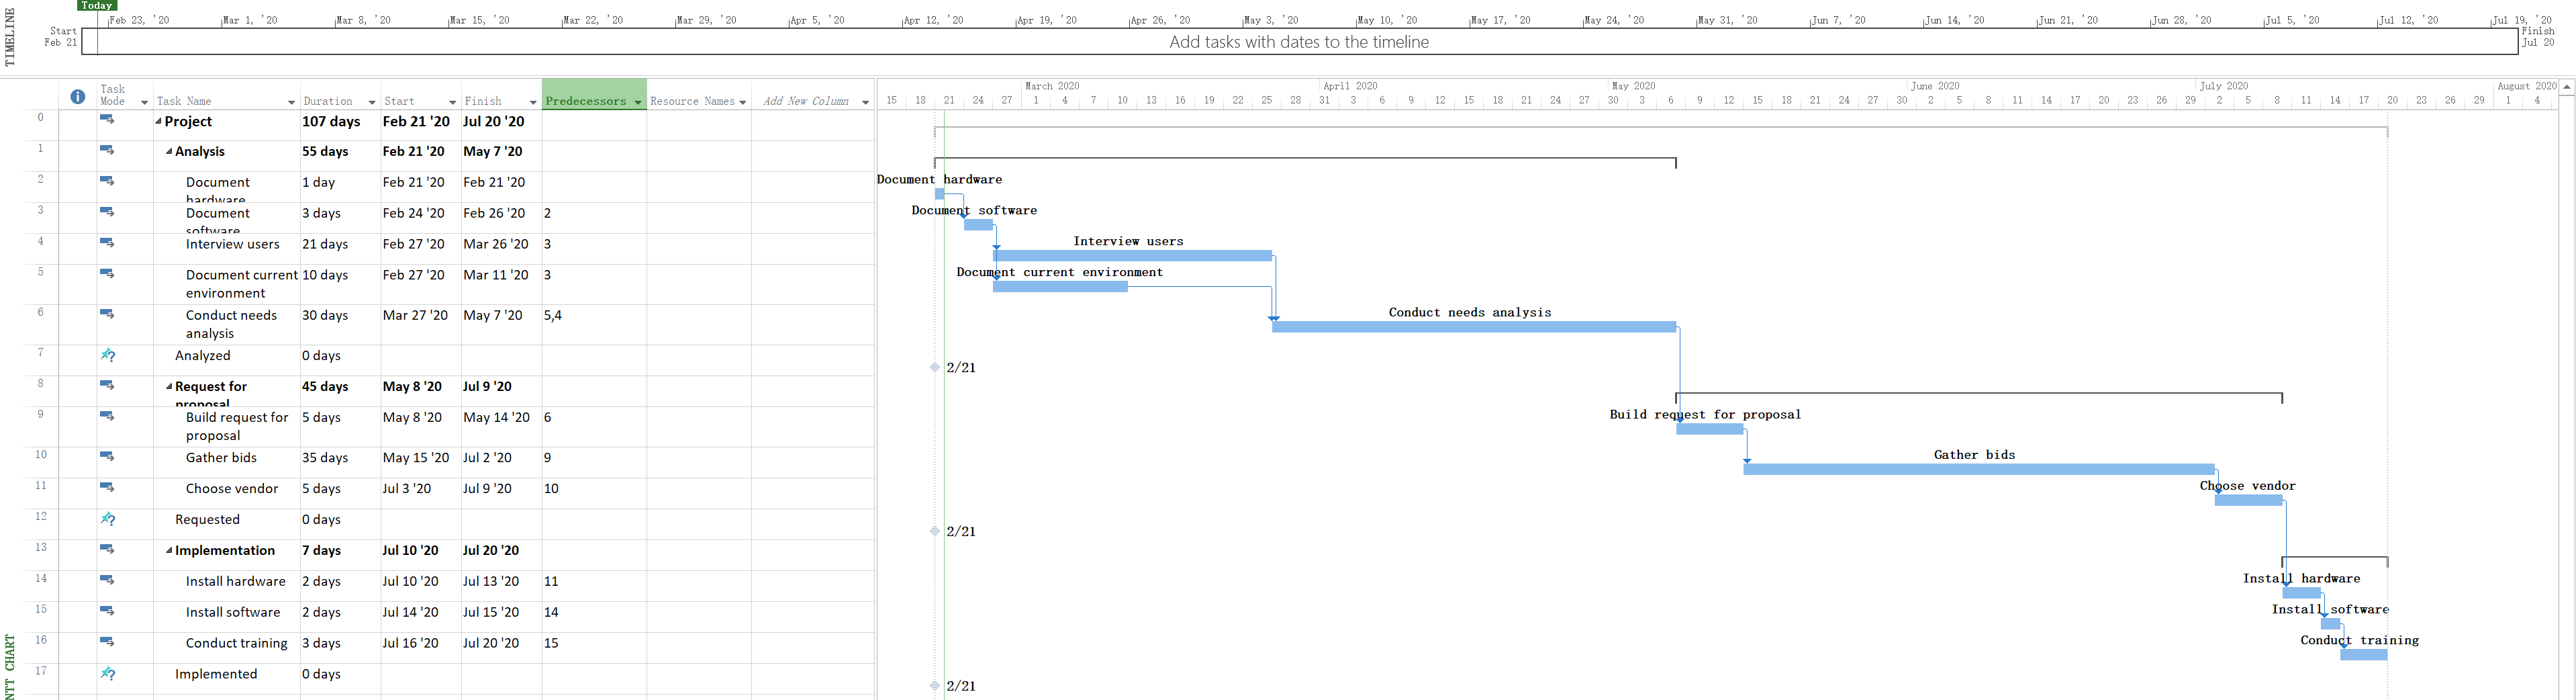
\includegraphics[width=1.0\textwidth]{./image/proj2}
    \caption{Gantt Chart 2}
\end{figure}

\noindent11) Considering Qingming Festival (Apr. 4–6), Labor Day(May 1–5) and The Dragon Boat Festival (June 25–27), the end time will delay to Jul. 28.
\begin{figure}[H]
    \centering
    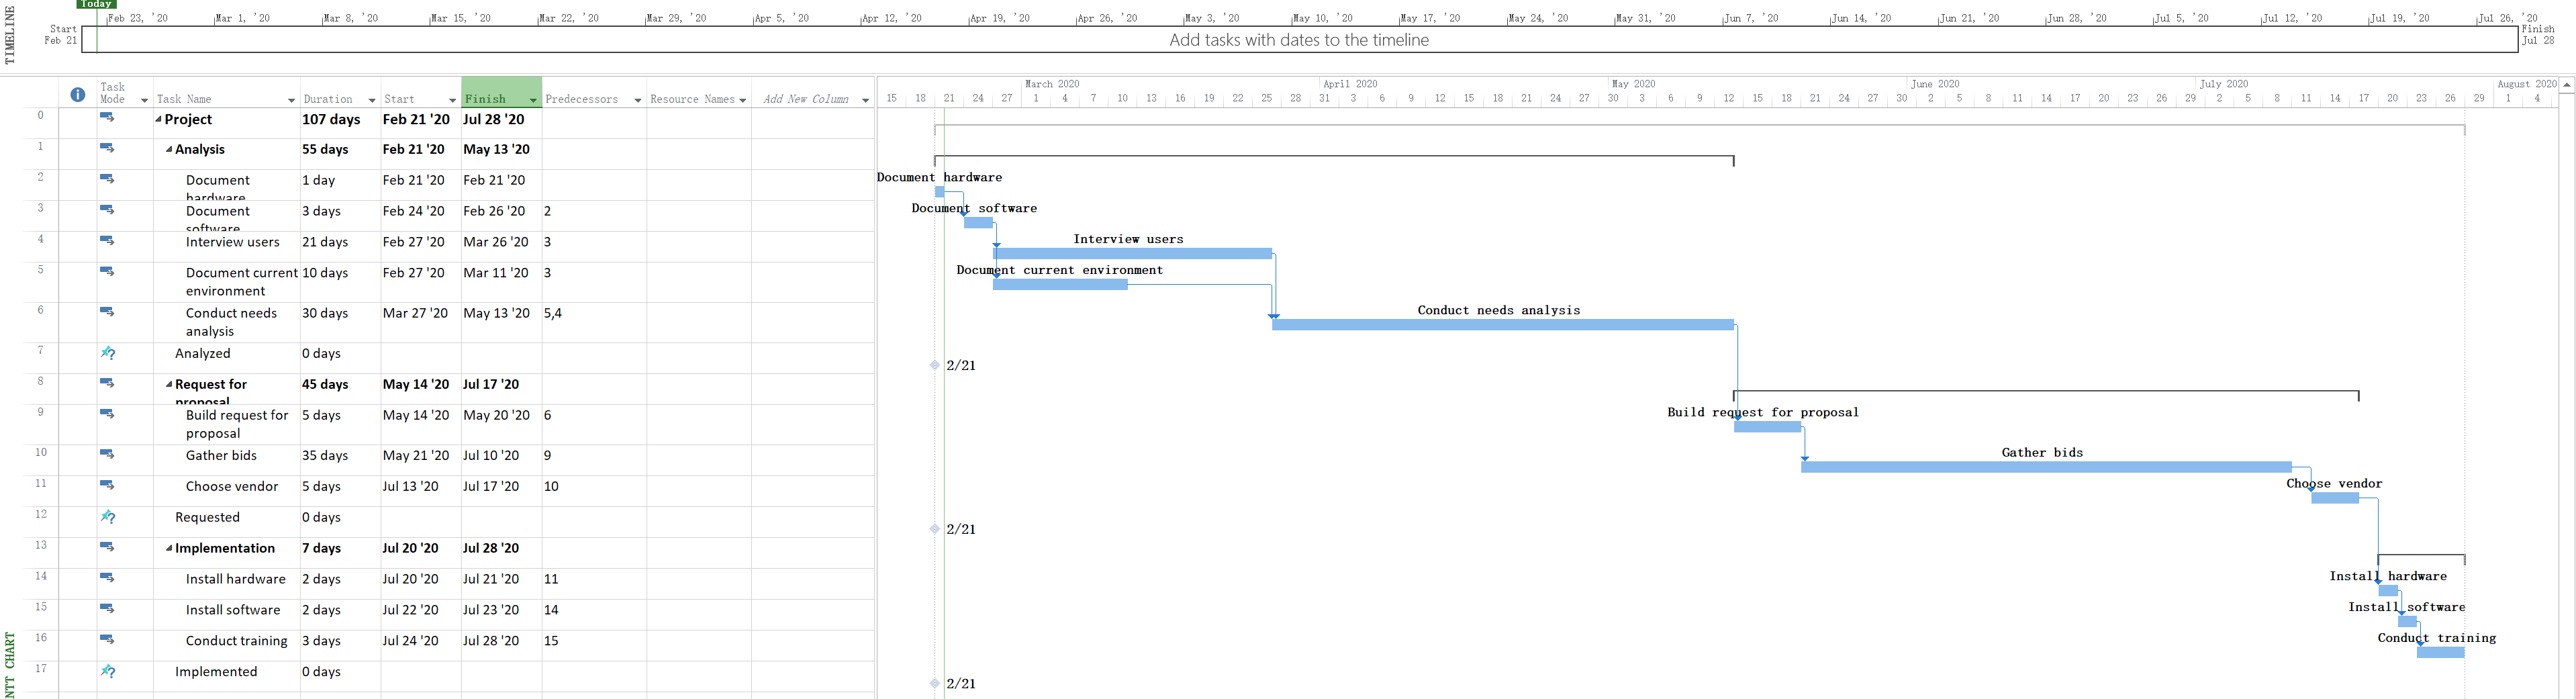
\includegraphics[width=1.0\textwidth]{./image/proj3}
    \caption{Gantt Chart 2}
\end{figure}


\section{Lab1}
\subsection{Description}

The project describe the process of software product development. There are 4 phases in the procedure: Requirements analysis, Design, Development and Deployment. 

\noindent Requirements analysis phase (7 days, Feb. 21-Jul. 9) contains "Communication and Documentation" and "Evaluation and Verification", When the latter one is finished, the Milestone "Requirements analysis completed" is reached.

\noindent Design analysis phase (25 days, Mar. 3-Apr. 10) contains "Design prototype" and "Design UI", When the two tasks are finished, the Milestone "Complete product design" is reached.

\noindent Development phase (40 days, Mar. 25-May 29) contains "Backend development", "Frontend development" and "Source merging and compiling". The prototype design is the prerequisite of backend development while the UI design is the prerequisite of frontend development. When frontend and backend sources are merged and compiled, the Milestone "Product development completed". 

\noindent Deployment phase (26 days, May 29-Jul. 9) contains "Public Beta Testing", "Product quality inspection" and "Product Release". The former tasks are the prerequisites of the latter tasks. When the product is released, the Milestone of "Officially launched product" is reached.


\begin{figure}[H]
    \centering
    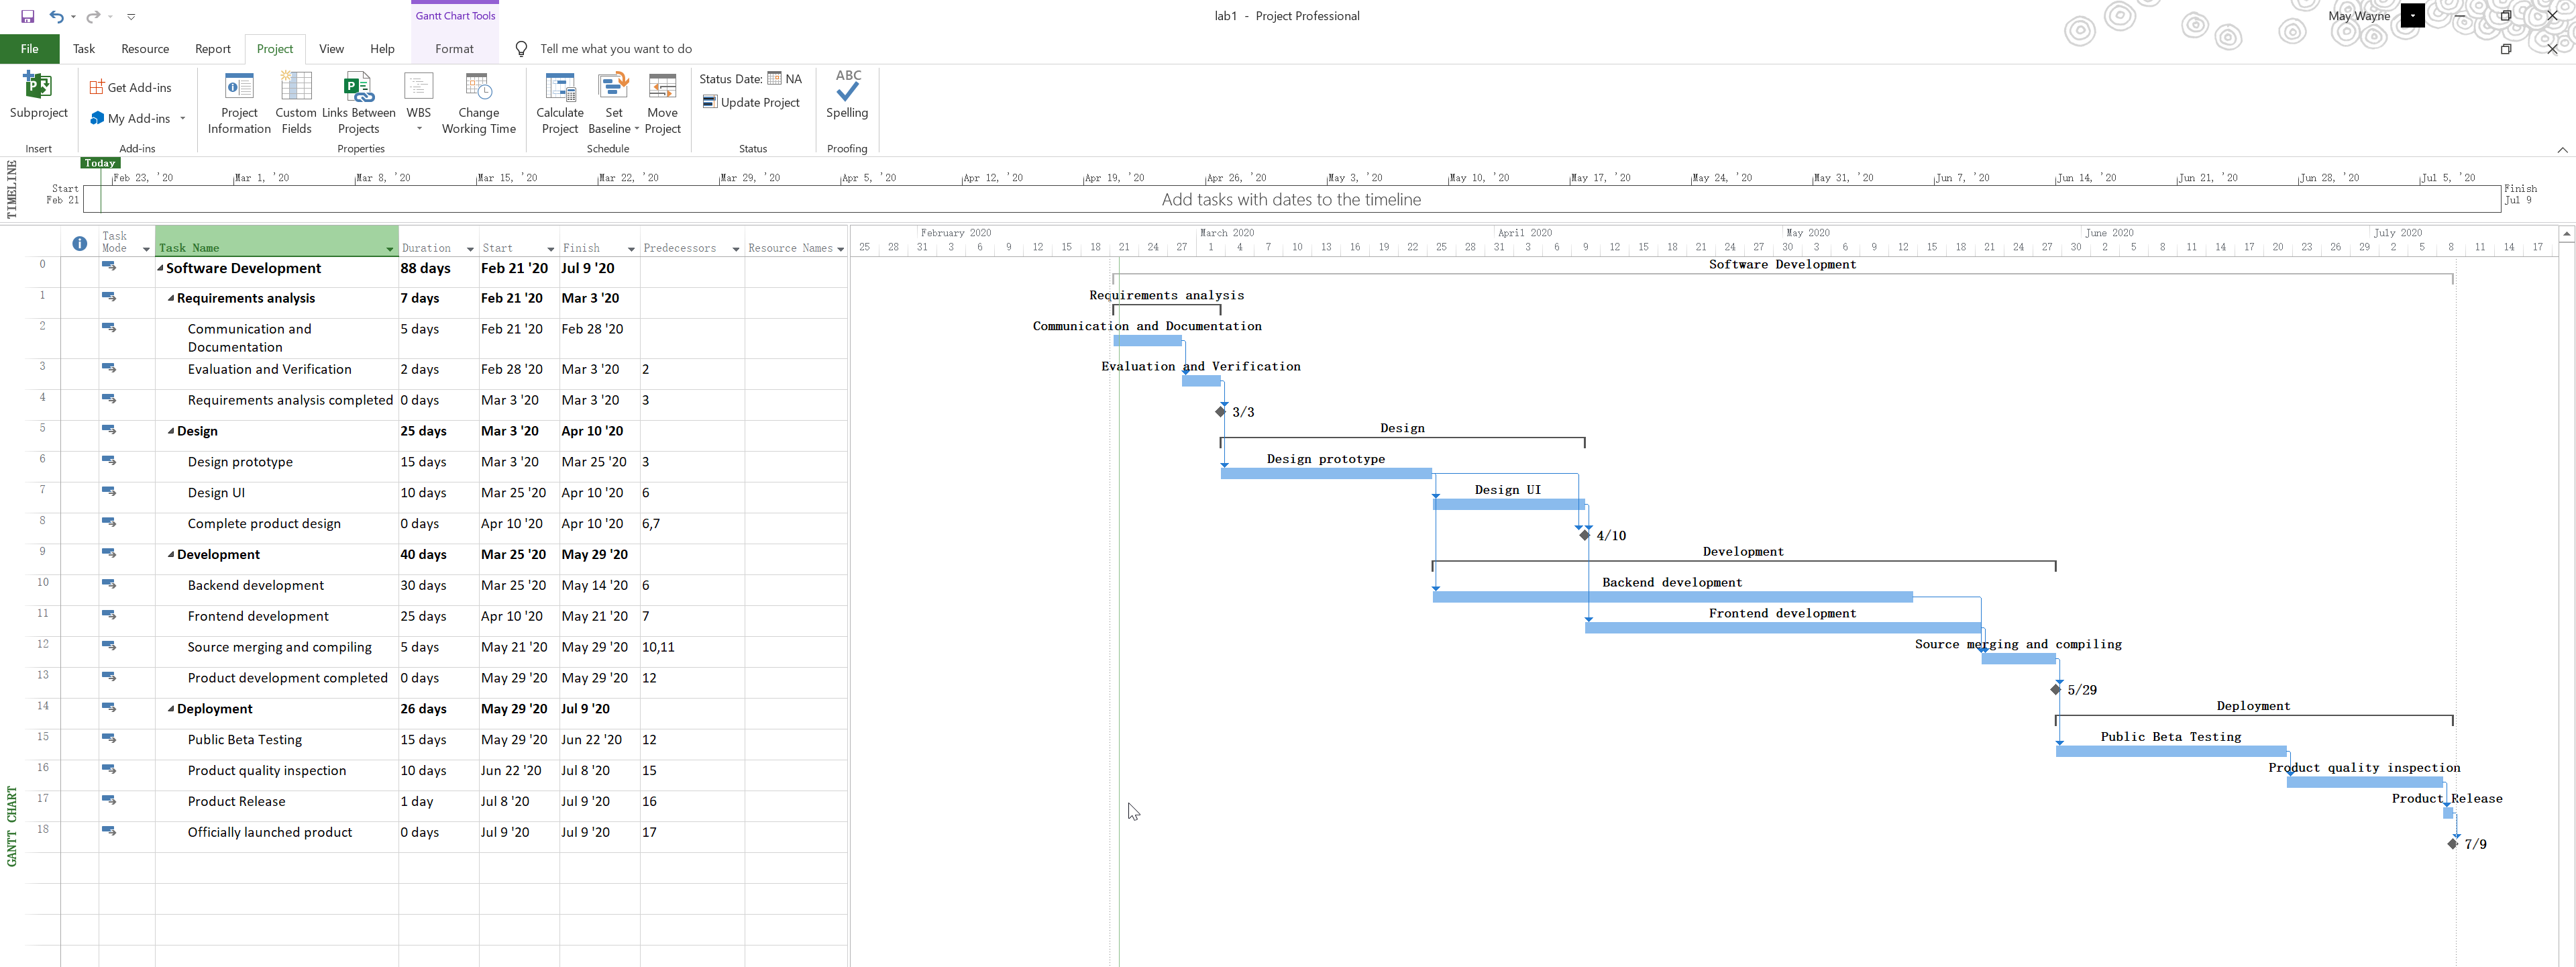
\includegraphics[width=1.0\textwidth]{./image/lab1-1}
    \caption{Gantt Chart of Software development}
\end{figure}

\subsection{Evidence of requirement 4}
Chinese public holidays within the project period are introduced. 

\begin{figure}[H]
    \centering
    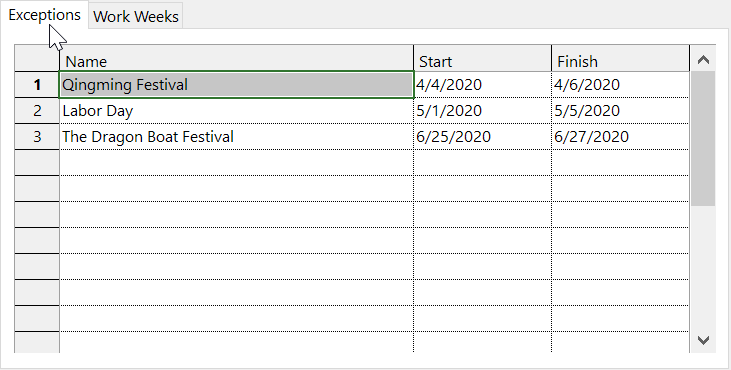
\includegraphics[width=1.0\textwidth]{./image/festivals}
    \caption{Chinese public holidays}
\end{figure}

The working hours are also set to Monday to Friday 8:30am-12:pm and 1:00pm-5:00pm.

\begin{figure}[H]
    \centering
    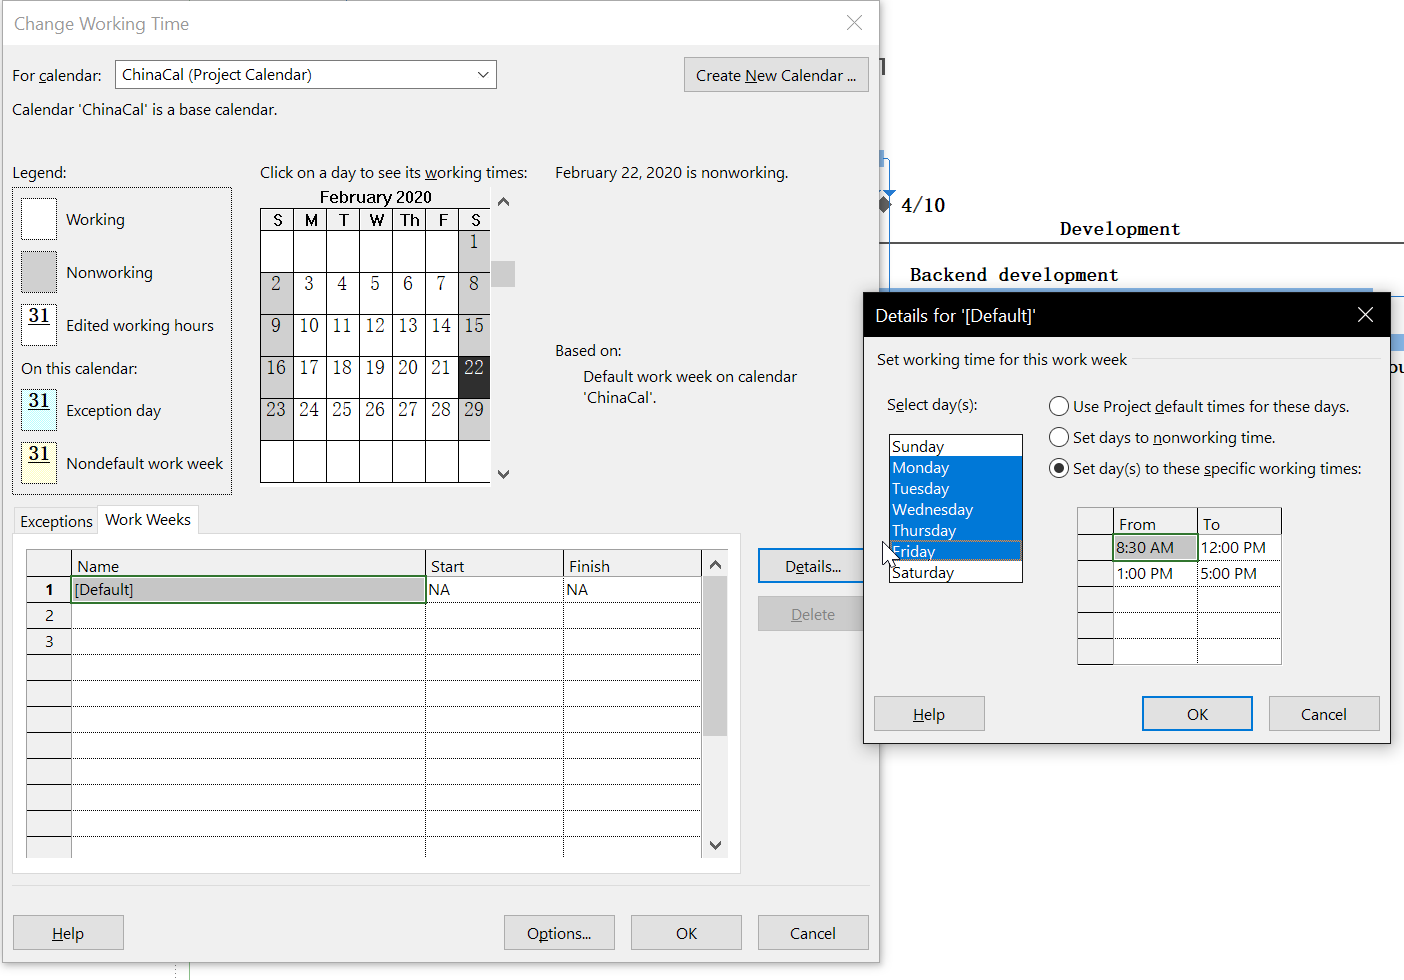
\includegraphics[width=0.5\textwidth]{./image/workinghours}
    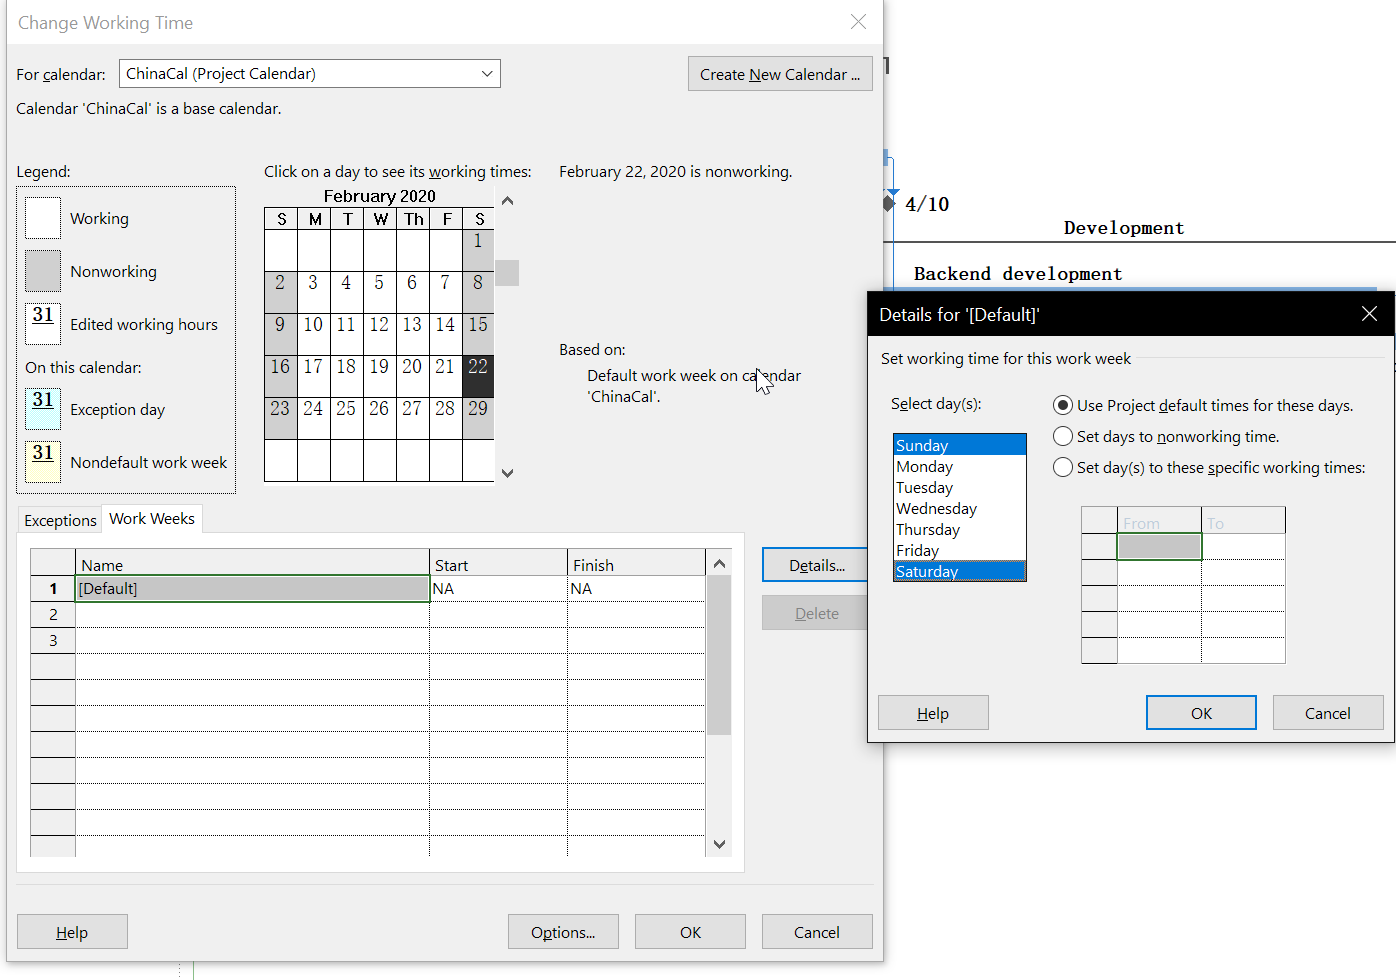
\includegraphics[width=0.5\textwidth]{./image/workinghours2}
    \caption{Working Hours}
\end{figure}




\end{document}
